\subsubsection{PartyMixer App}
\label{subsubsec:Software_PartyMixer_App}

Damit die App so benutzerfreundlich wie möglich ist, wurde sie in einem sehr schlichten Design erstellt. Das Design und die Funktionen erinnern an das Display des PartyMixers und helfen somit dem Kunden intuitiver damit arbeiten zu können. Es können in der App drei Dinge gemacht werden. Dabei wurde darauf geschaut, dass es sich niemals um Punkte handelt, welche vom App und Display gleichzeitig beeinflusst werden können. Somit wäre es zum Beispiel unpraktisch mit der App bereits erstellte Cocktails bearbeiten zu können, da man sich so mit der App und dem Display hinein pfuschen kann. Grundsätzlich gibt es zwei mögliche Einstellungen, welche vorgenommen werden können in der App und eine Information.\todo{Wo hinein pfuschen?} \\ 

Als Erstes muss eine Bluetooth-Verbindung mit dem PartyMixer hergestellt werden. Dazu kann man mit dem Button \flqq Bluetooth-Gerät wählen\frqq~ein Bluetoothgerät aus der eigenen Bluetooth-Liste gewählt werden. Beim Loslassen des Buttons erscheint somit eine Auswahlliste. Achtung: Das erste Mal muss das Gerät in den Geräteeinstellungen Verbunden werden, bevor es in der Liste erscheint. Nach dem das Gerät mit der Maschine verbunden ist, gelangt man mittels Tastendruck auf \flqq RFID\frqq~in die RFID-Einstellung, wo man einem spezifischen RFID-Tag ein Getränk zuweisen kann. Per Klick auf \flqq RFID-Tag wählen\frqq~erscheint eine Scrollbare Liste mit 10 Tag's, wobei man seinen erhaltenen RFID-Tag auswählen kann. Nach der Auswahl schliesst sich die Liste wieder und dieser wird über dem Button angezeigt. Als nächstes muss man das gewünschte Getränk auswählen, welches man dem Tag zuordnen möchte. Dazu erscheint beim Klicken auf \flqq Getränk wählen\frqq~die aktuelle Cocktailliste, welche in der Maschine gespeichert ist. Auch hier verschwindet die Liste beim Klick auf einen Cocktail und man gelangt zurück. Das Getränk wird wie der Tag über dem Button angezeigt. Ist man mit der Auswahl zufrieden, so kann man den Vorgang mit Speichen abschliessen und das Getränk ist dem Tag zugeordnet. Man kann nun weitere Tag's zuordnen oder mit dem Button \flqq Zurück\frqq~zurück ins Hauptmenü gehen.
Die Menübildschirme sind in Abbildung \ref{fig:AppRFID} zu sehen.\\

\begin{figure}[h!]
	\centering
	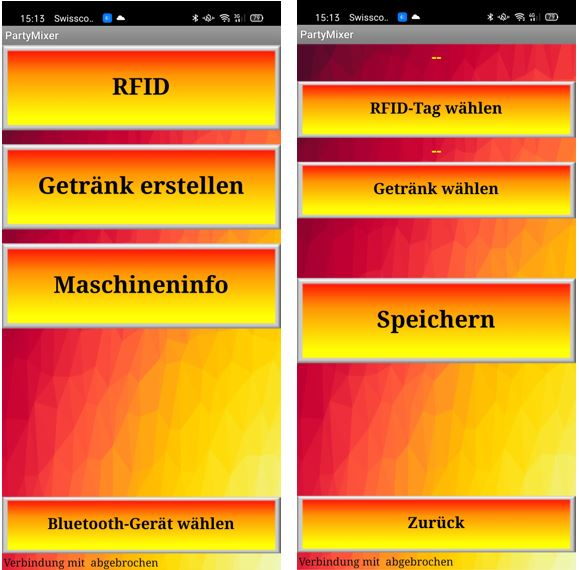
\includegraphics[width=0.4\textwidth]{graphics/AppRFID}
	\caption{RFID Einstellungen der App}
	\label{fig:AppRFID}
\end{figure}

Eine weitere Einstellung, welche man vornehmen kann, ist die Erstellung eines eigenen Getränks, welches auf der Maschine gespeichert werden soll. Möchte man dies umsetzen, so gelangt man mit den Klick auf \flqq Getränk erstellen\frqq~in die Namensvergabe, wo man dem neuen Cocktail einen Namen geben kann. Wenn kein Name eingetippt wird, so ist der Button \flqq Weiter\frqq~ohne Funktion. Mit \flqq Zurück\frqq~gelangt man erneut ins Hauptmenü. Per Klick auf das Textfeld erscheint die Telefontastatur und es kann ein Name eingegeben werden. Mit \flqq Weiter\frqq~wird dieser gespeichert und man kommt in die Erstellungsanzeige. Da mit App Inventor keine dynamischen Buttons oder Slider erstellbar sind, musste nach einer anderen Lösung gesucht werden. Deshalb werden die Zutaten einzeln Ausgewählt. Mit Klick auf \flqq Zutaten\frqq~erscheint die aktuelle Zutatenliste, wobei man seine erste Zutat auswählen kann, welche im Cocktail enthalten sein soll. Bei Auswahl verschwindet die Liste und die Zutat wird über dem Button angezeigt. Mit dem Slider kann nun in 5\% Schritten die gewünschte Menge eingestellt werden, welche im Cocktail enthalten sein soll. Bei Klick auf \flqq Gewählte Zutat Hinzufügen\frqq~ wird die Auswahl abgespeichert, der Slider fällt auf 0 und es wird bei \flqq Gewähltes Mischverhältnis\frqq~eine Liste angezeigt mit dem bereits getroffenen Einstellungen. Diesen Vorgang kann man so oft wiederholen, bis man 100\% eingestellt hat. Wird weniger als 100\% eingestellt, so erscheint bei Kick auf \flqq Fertig\frqq~ eine Meldung, dass bitte 100\% eingestellt werden soll. Wird mit dem Slider mehr hinzugefügt, so dass mehr als 100\% entsteht, so fällt dieser auf die verbleibende Menge bis 100\% zurück und man kann diesen Wert hinzufügen. Will man eine Auswahl ändern, so muss man lediglich die zu ändernde Flüssigkeit auswählen und den neuen Wert abspeichern. Sind 100\% eingestellt, so kann man mit \flqq Fertig\frqq~den Cocktail abspeichern und man gelangt wieder ins Hauptmenü. Die Menübildschirme sind hierbei in Abbildung \ref{fig:AppErstellen} zu sehen.\\

\begin{figure}[h!]
	\centering
	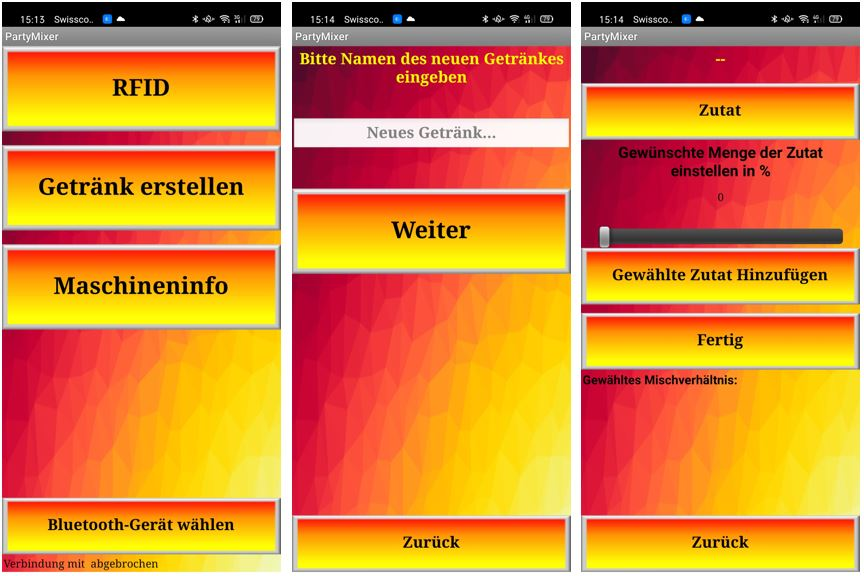
\includegraphics[width=0.6\textwidth]{graphics/AppErstellen}
	\caption{Getränk erstellen in der App}
	\label{fig:AppErstellen}
\end{figure}

\newpage

Mit einem Klick auf \flqq Maschineninfo\frqq~im Hauptmenu gelangt man in die Infoanzeige, wo einem Informationen zur Maschine angezeigt werden. Mit einem Klick auf \flqq Zurück\frqq~gelangt man erneut ins Hauptmenu. Die Menubildschirme dazu sind in Abbildung \ref{fig:AppInfo} zu sehen.

\begin{figure}[h!]
	\centering
	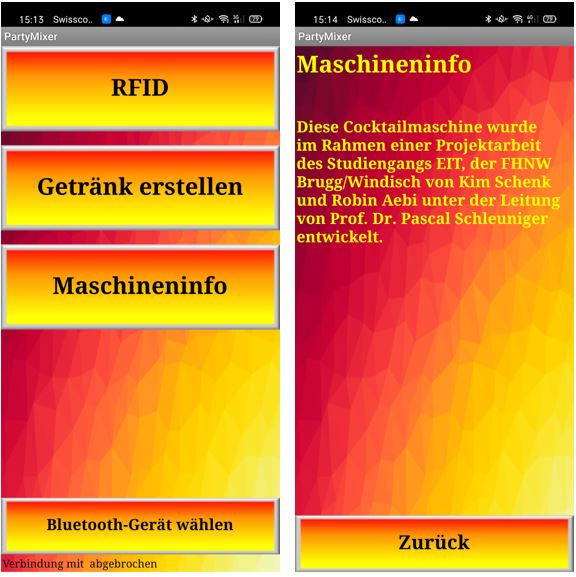
\includegraphics[width=0.4\textwidth]{graphics/AppInfo}
	\caption{Infoanzeige der App}
	\label{fig:AppInfo}
\end{figure}

 
